% 水压力例子(a)
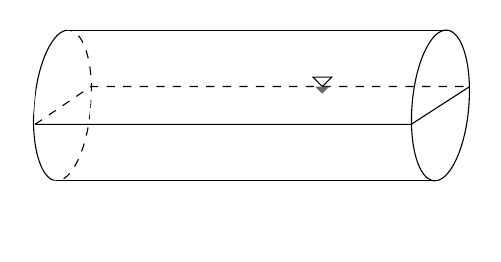
\begin{tikzpicture}[scale=0.6]
  % \draw [help lines] (-1,-3) grid (9,3);

  % 左椭圆
  \begin{scope}
    \clip[rotate=-5] (-0.6,-1.6) rectangle (0,1.6);
    \draw[rotate=-5] (0,0) ellipse [x radius=0.6cm,y radius=1.6cm];
  \end{scope}
  \begin{scope}
    \clip[rotate=-5] (0,-1.6) rectangle (0.6,1.6);
    \draw[dashed,rotate=-5] (0,0) ellipse [x radius=0.6cm,y radius=1.6cm];
  \end{scope}

  % 上下边框
  \draw (0.139,1.593) -- (8.139,1.593);
  \draw (-0.139,-1.593) -- (7.861,-1.593);

  % 水面
  \draw (-0.58,-0.4) -- (7.38,-0.4) -- (8.62,0.4);
  \draw[dashed] (-0.58,-0.4) -- (0.6,0.4) -- (8.62,0.4);

  \draw (5.5,0.4) -- (5.3,0.6) -- (5.7,0.6) -- (5.5,0.4);
  \path[fill=black!60] (5.5,0.25) -- (5.35,0.4) -- (5.65,0.4) -- (5.5,0.25);

  % 右椭圆
  \draw[rotate around={-5:(8,0)}] (8,0) ellipse [x radius=0.6cm,y radius=1.6cm];

  % 空白,提升高度,底部的 padding
  \draw[white] (0,-2.7) -- (0.01,-2.7);
\end{tikzpicture}
